\documentclass{article}

\usepackage{graphicx}
\usepackage{color}
\usepackage{array}
\usepackage{longtable}
\usepackage{comment} 
\usepackage{hyperref}

\begin{document}

\title{jStar Eclipse tutorial} 
\maketitle 


\section{Installation}

Prerequisites:
\begin{itemize}
   \item JDK 6 (not JRE since it does not have a compiler needed for annotation processing). You can specify it in eclipse.ini:\\\\
Windows Example\\
-vm\\
C:\textbackslash Java\textbackslash JDK\textbackslash 1.6\textbackslash bin\textbackslash javaw.exe\\

Linux Example\\
-vm\\
/opt/sun-jdk-1.6.0.02/bin/java\\

Mac Example\\
-vm\\
/System/Library/Frameworks/JavaVM.framework/Versions/1.6.0/Home/bin/java\\

For more information go to \href{http://wiki.eclipse.org/Eclipse.ini}{http://wiki.eclipse.org/Eclipse.ini}

\end{itemize}
Two ways:
\begin{enumerate}
\item Add the jar file \textbf{jar\_files/plugins/com.jstar.eclipse\_1.0.0.x.jar} to \texttt{eclipse/dropins/} folder and restart Eclipse.
\item {\color{red} Need to create an update site.}
\end{enumerate}

\section{Configuration}

On Windows with cygwin:

Go to Windows $\rightarrow$ Preferences $\rightarrow$ jStar Configuration and set the required directories.\\

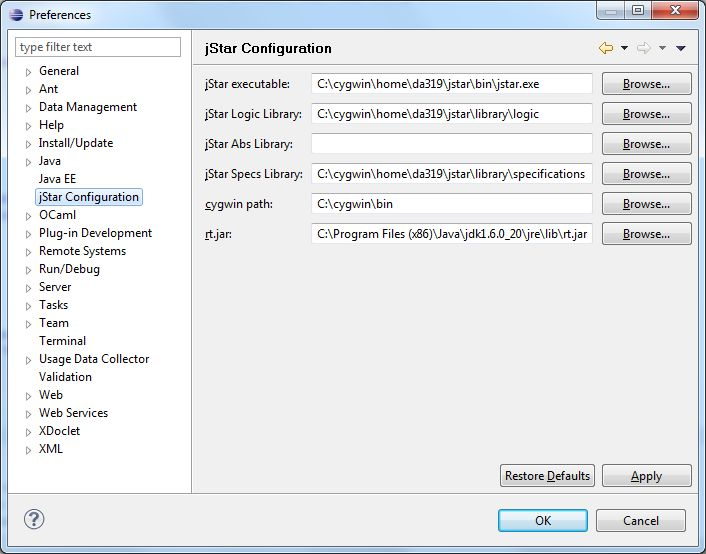
\includegraphics[width=4in]{images/preferences.jpg}

\section{Verification}
You can verify source file by selecting \texttt{Verify with jStar} from the context menu or the main toolbar. 

By selecting \texttt{Verify with jStar Configurations...}, you can indicate the location of specification, logic and abstraction rules.\\

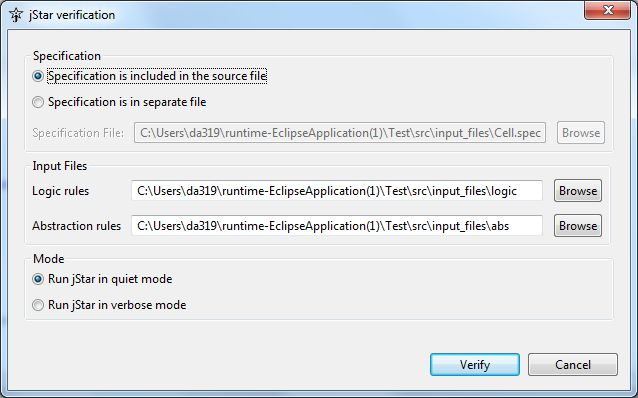
\includegraphics[width=4in]{images/verificationWindow.jpg}

\subsection*{Specification in source file}

If you want to write specification in the source file, you need to add annotations.jar (can be found in com.jstar.eclipse/jar files/annotations) to your project Java Build Path.

\subsection*{Annotations}

\begin{itemize}
\item \texttt{@Import} has one element \texttt{String[] value}. This annotation can be used to annotate only type declarations.
\item \texttt{@Predicate} is used for \texttt{define} and \texttt{export} statements. It has three elements: \texttt{String predicate}, \texttt{String formula}, \texttt{DefinitionType type}. \texttt{DefinitionType} is enum with two values \texttt{Define} and \texttt{Export}.  The default value of type is \texttt{DefinitionType.Define}. This annotation can be used to annotate only type declarations.
\item \texttt{@Predicates} is used if you want to have more than one  \texttt{define} and/or \texttt{export} statements. It has one element \texttt{Predicate[] value}. This annotation can be used to annotate only type declarations.
\item \texttt{@InitSpec} is a (dynamic / both static and dynamic) specification for constructor which is not explicitly defined in the source code. It has two elements: \texttt{String pre}, \texttt{String post}. This annotation can be used to annotate only type declarations.
\item \texttt{@InitSpecs} is (dynamic / both static and dynamic) specifications which are conjuncted with \texttt{also} for constructor which is not explicitly defined in the source code. It has one element \texttt{InitSpec[] value}. This annotation can be used to annotate only type declarations.
\item \texttt{@InitSpecStatic} is a static specification for constructor which is not explicitly defined in the source code. It has two elements: \texttt{String pre}, \texttt{String post}. This annotation can be used to annotate only type declarations.
\item \texttt{@InitSpecsStatic} is static specifications which are conjuncted with \texttt{also} for constructor which is not explicitly defined in the source code. It has one element \texttt{InitSpecStatic[] value}. This annotation can be used to annotate only type declarations.
\item \texttt{@Spec} is a (dynamic / both static and dynamic) specification for a method or a constructor. It has two elements: \texttt{String pre}, \texttt{String post}. This annotation can be used to annotate only method and constructor declarations.
\item \texttt{@Specs} is (dynamic / both static and dynamic) specifications which are conjuncted with \texttt{also} for a method or a constructor. It has one element: \texttt{Spec[] value}. This annotation can be used to annotate only method and constructor declarations.
\item \texttt{@SpecStatic} is a static specification for a method or a constructor. It has two elements: \texttt{String pre}, \texttt{String post}. This annotation can be used to annotate only method and constructor declarations.
\item \texttt{@SpecsStatic} is static specifications which are conjuncted with \texttt{also} for a method or a constructor. It has one element: \texttt{SpecStatic[] value}. This annotation can be used to annotate only method and constructor declarations.
\end{itemize}


Examples of annotations in the source code:\\
\begin{longtable}{ m{7cm} | m{5cm} }
Annotation in source file & Generated specification file \\
\hline
\begin{verbatim}
@Import("Spec.spec")
\end{verbatim}
& 
\begin{verbatim}
import("Spec.spec");
\end{verbatim}
\\
\begin{verbatim}
@Import({"Spec1.spec", "Spec2.spec"})
\end{verbatim}
& 
\begin{verbatim}
import("Spec1.spec");
import("Spec2.spec");
\end{verbatim}
\\
\begin{verbatim}
@Predicate(
   predicate = "P(x)", 
   formula = "F(x)"
)
\end{verbatim} 
&
\begin{verbatim}
define P(x) as F(x);
\end{verbatim}
\\
\begin{verbatim}
@Predicate(
   predicate = "P(x)", 
   formula = "F(x)", 
   type = DefinitionType.Export
)
\end{verbatim}  
&
\begin{verbatim}
export P(x) as F(x);
\end{verbatim}\\
\begin{verbatim}
@Predicates({
   @Predicate(
      predicate = "P1(x)", 
      formula = "F1(x)", 
      type = DefinitionType.Export
   ),
   @Predicate(
      predicate = "P2(x)", 
      formula = "F2(x)"
   )
})
\end{verbatim} 
& 
\begin{verbatim}
export P1(x) as F1(x);
define P2(x) as F2(x);
\end{verbatim}
\\
\begin{verbatim}
@InitSpec(
   pre = "precondition", 
   post = "postcondition"
)
\end{verbatim}
&
\begin{verbatim}
void <init>() :
   { precondition }
   { postcondition }
\end{verbatim}
\\
\begin{verbatim}
@InitSpecs({
   @InitSpec(
      pre = "precondition 1", 
      post = "postcondition 1"
   ),
   @InitSpec(
      pre = "precondition 2",
      post = "postcondition 2"
   )
})
\end{verbatim}
&
\begin{verbatim}
void <init>() :
   { precondition 1 }
   { postcondition 1 }
   andalso
   { precondition 2 }
   { postcondition 2 }
\end{verbatim}
\\
\begin{verbatim}
@InitSpecStatic(
   pre = "precondition",
   post = "postcondition"
)
\end{verbatim}
&
\begin{verbatim}
void <init>() static :
   { precondition }
   { postcondition }
\end{verbatim}
\\
\begin{verbatim}
@InitSpecsStatic({
   @InitSpecStatic(
      pre = "precondition 1", 
      post = "postcondition 1"
   ),
   @InitSpecStatic(
      pre = "precondition 2",
      post = "postcondition 2"
   )
})
\end{verbatim}
&
\begin{verbatim}
void <init>() static :
   { precondition 1 }
   { postcondition 1 }
   andalso
   { precondition 2 }
   { postcondition 2 }
\end{verbatim}
\\
\begin{verbatim}
@Spec(
   pre = "precondition", 
   post = "postcondition"
)
\end{verbatim}
\it{method declaration}
&
{\it method declaration} \texttt{:}
\begin{verbatim}
   { precondition }
   { postcondition }
\end{verbatim}
\\
\begin{verbatim}
@Specs({
   @Spec(
      pre = "precondition 1", 
      post = "postcondition 1"
   ),
   @Spec(
      pre = "precondition 2", 
      post = "postcondition 2"
   )
})
\end{verbatim}
\it{method declaration}
&
{\it method declaration} \texttt{:}
\begin{verbatim}
   { precondition 1 }
   { postcondition 1 }
   andalso
   { precondition 2 }
   { postcondition 2 }
\end{verbatim}
\\
\begin{verbatim}
@SpecStatic(
   pre = "precondition", 
   post = "postcondition"
)
\end{verbatim}
\it{method declaration}
&
{\it method declaration} \texttt{static :}
\begin{verbatim}
   { precondition }
   { postcondition }
\end{verbatim}
\\
\begin{verbatim}
@SpecsStatic({
   @SpecStatic(
      pre = "precondition 1", 
      post = "postcondition 1"
   ),
   @SpecStatic(
      pre = "precondition 2", 
      post = "postcondition 2"
   )
})
\end{verbatim}
\it{method declaration}
&
{\it method declaration} \texttt{static :}
\begin{verbatim}
   { precondition 1 }
   { postcondition 1 }
   andalso
   { precondition 2 }
   { postcondition 2 }
\end{verbatim}
\end{longtable}

\subsection* {Verification errors}

In case there are some verification errors, you can see error messages in console. The lines in source code where the problem appeared are annotated as squiggly marks.\\

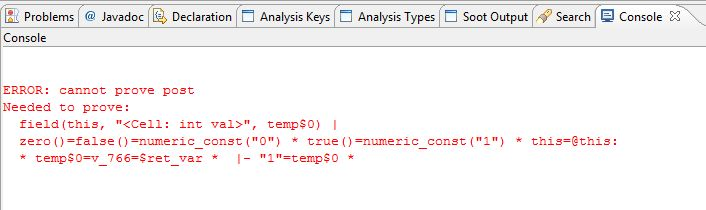
\includegraphics[width=4in]{images/console.jpg}\\

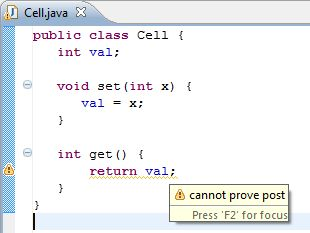
\includegraphics[width=2in]{images/marker.jpg}



\end{document}